\documentclass{article}

% file's preambule
%%%%%%%%%%%%%%%%%%%



% connect packages
\usepackage[T2A]{fontenc}
\usepackage[utf8]{inputenc}
\usepackage[english]{babel}
\usepackage{hyperref}     % ТАК_НУЖНО
\hypersetup{unicode=true} % ТАК_НУЖНО
\usepackage{amsmath}
\usepackage{amssymb,textcomp, esvect,esint}
\usepackage{amsfonts}
\usepackage{amsthm}
\usepackage{graphicx}
\usepackage{indentfirst}
\usepackage{xcolor}
% \usepackage{enumitem} %--- ломал нумерацию!?

\usepackage{graphicx}
\usepackage{booktabs}
\usepackage{caption}
\usepackage{listings}
\usepackage{tikz}
\usepackage{xcolor}



\usepackage{media9}
\usepackage{animate}
\usepackage{threeparttable}
\usepackage{pifont}


\usepackage{import}
\usepackage{xifthen}
\usepackage{pdfpages}
\usepackage{transparent}

\usepackage[skip=1pt]{caption}

% create environment

\newtheorem{to_thr}{Thr}[section]
\newtheorem{to_suj}[to_thr]{Suj}
\newtheorem{to_lem}[to_thr]{Lem}
\newtheorem{to_com}[to_thr]{Com}
\newtheorem{to_con}[to_thr]{Con}
\theoremstyle{definition}
\newtheorem{to_def}[to_thr]{Def}


\newenvironment{itemize*}
{
    \begin{itemize}
        \setlength{\itemsep}{1pt}
        \setlength{\parskip}{1pt}}
    {\end{itemize}
}

\newenvironment{enumerate*}
{
    \begin{enumerate}
        \setlength{\itemsep}{1pt}
        \setlength{\parskip}{1pt}}
    {\end{enumerate}
}

\newenvironment{description*}
{
    \begin{description}
        \setlength{\itemsep}{1pt}
        \setlength{\parskip}{1pt}}
    {\end{description}
}


\newenvironment{hw1}
{
    \phantom{42}

    \noindent
    \textbf{Домашнее задание:} \hrulefill
    % \vspace{-2mm}
    % \begin{enumerate*}

}
{
    % \end{enumerate*}
    \vspace{2mm}
    \hrule

    \phantom{42}
}


\newenvironment{hw2}
{
    \phantom{42}

    \noindent
    \textbf{Домашнее задание:} \hrulefill
    \vspace{-2mm}
    \begin{enumerate*}

}
{
    \end{enumerate*}
    \hrule

    \phantom{42}
}

% document palette
\definecolor{ugreen}{RGB}{0, 100, 0}
\definecolor{ured}{RGB}{220, 0, 0}
\definecolor{ugray}{RGB}{90, 90, 90}

% \newcommand{\red}[1]{\textcolor{ured}{#1}}
% \newcommand{\green}[1]{\textcolor{ugreen}{#1}}


\definecolor{grey}{HTML}{666666}
\definecolor{linkcolor}{HTML}{0000CC}
\definecolor{urlcolor}{HTML}{006600}
\hypersetup{
    pdfstartview=FitH,  
    linkcolor=linkcolor,
    urlcolor=urlcolor, 
    colorlinks=true,
    citecolor=blue}

% add (renew) commands
% add (renew) commands

\renewcommand{\Im}{\mathop{\mathrm{Im}}\nolimits}
\renewcommand{\Re}{\mathop{\mathrm{Re}}\nolimits}

\renewcommand{\d}{\, d}
\renewcommand{\leq}{\leqslant}
\renewcommand{\geq}{\geqslant}
\renewcommand{\l}{\left}
\renewcommand{\r}{\right}

\newcommand{\vc}[1]{\mbox{\boldmath $#1$}}
\newcommand{\T}{^{\text{T}}}


\newcommand{\diag}{\mathop{\mathrm{diag}}\nolimits}
\newcommand{\cl}{\mathop{\mathrm{cl}}\nolimits}
\newcommand{\grad}{\mathop{\mathrm{grad}}\nolimits}
\renewcommand{\div}{\mathop{\mathrm{div}}\nolimits}
\newcommand{\rot}{\mathop{\mathrm{rot}}\nolimits}
\newcommand{\Ker}{\mathop{\mathrm{Ker}}\nolimits}
\newcommand{\Spec}{\mathop{\mathrm{Spec}}\nolimits}
\newcommand{\sign}{\mathop{\mathrm{sign}}\nolimits}
\newcommand{\tr}{\mathop{\mathrm{tr}}\nolimits}
\newcommand{\rg}{\mathop{\mathrm{rg}}\nolimits}


\newcommand{\DS}{\mathcal D\left(\mathbb{R}\right)}
\newcommand{\QED}{\textnormal{Q. E. D.}}
\newcommand{\dseq}{\overset{\mathcal D'}{=}}
\newcommand{\dto}{\overset{\mathcal D'}{\to}}


\newcommand{\const}{\text{const}}
\newcommand{\xmark}{\ding{55}}


\newenvironment{uproof}{
% \begin{comment}
\par \color{ugray}
\begin{proof}[$\triangle$]
}{
\end{proof} \par
% \end{comment}
}


\newcommand{\bhat}{\overset{\text{\scalebox{0.8}[0.5]{\rotatebox[origin=c]{180}{$\wedge$}}}}}

\newcommand{\cf}[1]{\text{\raisebox{1.5pt}{$\scalebox{1.3}{$\chi$}$}}_{#1}}

\newcommand{\supp}{\mathop{\mathrm{supp}}\nolimits}
\newcommand{\si}{\mathop{\mathrm{Si}}\nolimits}

\newcommand{\rr}{\rightrightarrows}

% \newcommand{\sbsnum}[2]{
%     \setcounter{subsection}{\the\numexpr #1 - 1 \relax}
%     \subsection{#2}
% }

% Секции и сабсекции
% \definecolor{darkblue}{HTML}{000099}
% \newcommand{\sbs}[1]{\subsection{\textcolor{darkblue}{#1}}}
% \renewcommand{\sec}[1]{\section{\textcolor{darkblue}{#1}}}
\newcommand{\sbs}[2]{
\setcounter{subsection}{\numexpr #1 - 1 \relax}
    \textcolor{ugreen}{
        \subsection{#2}
        }
}



% add page header
% add page header

\pagestyle{fancy}
\fancyhf{}
\fancyhead[RE,LO]{\textsc{Ф\raisebox{-1.5pt}{и}з\TeX}}
\fancyhead[LE,RO]{Ж\raisebox{-1.5pt}{и}К}
\fancyhead[CO,CE]{\leftmark}
\fancyfoot[LE,RO]{\textcolor{grey}{\texttt{\thepage}}}



% matrixes shortcuts 
% \newcommand{\dmat}[4]{
  \ifthenelse{
    \equal{#1}{3}
  }{
\begin{pmatrix}
    #2 & 0 & 0 \\
    0 & #3 & 0 \\
    0 & 0 & #4 \\
\end{pmatrix}
  }{
  \ifthenelse{
      \equal{#1}{2}
    }{
  \begin{pmatrix}
      #2 & 0 \\
      0 & #3 \\
  \end{pmatrix}
    }{
      \text{\textcolor{red}{error}}
    }
  }
}

\newcommand{\skmat}[4]{
  \ifthenelse{
    \equal{#1}{3}
  }{
\begin{pmatrix}
    0 & -#4 & #3 \\
    #4 & 0 & -#2 \\
    -#3 & #2 & 0 \\
\end{pmatrix}
  }{
  \ifthenelse{
      \equal{#1}{2}
    }{
  \begin{pmatrix}
      0 & #2 \\
      -#2 & 0 \\
  \end{pmatrix}
    }{
      \text{\textcolor{red}{error}}
    }
  }
}

% additional symbols and commands


\DeclareRobustCommand{\tmpsim}{ %%%%%%%%%%%%%% ~ < %%%%%%%%%%%%%%%%%%%
  \mathbin{\text{
      \raisebox{-1pt}{
            \hspace{-4.5pt} \rotatebox{-26}{\scalebox{0.8}[0.7]{$\sim$}}
        }
  }}
}
\def\lesim{{
    \setbox0\hbox{$\ <\ $}
    \rlap{\hbox to \wd0{\hss$\tmpsim$\hss}}\box0
}}
%%%%%%%%%%%%%%%%%%%%%%%%%%%%%%%%%%%%%%%%%%%%%%%%%%%%%%%%%%%%%%%%%%%%%%


\def\letuscom{%%%%%%%%%%%%%%%%%%%%%% ПУСТЬ %%%%%%%%%%%%%%%%%%%%%%%%%%
\mathord{\setbox0=\hbox{$\exists$}%
     \hbox{\kern 0.125\wd0%
           \vbox to \ht0{%
              \hrule width 0.75\wd0%
              \vfill%
              \hrule width 0.75\wd0}%
           \vrule height \ht0%
           \kern 0.125\wd0}%
   }%
}
\newcommand{\letus}{\raisebox{-1.2pt}{$\letuscom$}}
%%%%%%%%%%%%%%%%%%%%%%%%%%%%%%%%%%%%%%%%%%%%%%%%%%%%%%%%%%%%%%%%%%%%%%


\usepackage{arydshln} %%%%%%%%%%%%%%% ЛИНИИ В МАТРИЧКЕ %%%%%%%%%%%%%%%
\makeatletter
  \renewcommand*\env@matrix[1][*\c@MaxMatrixCols c]{%
    \hskip -\arraycolsep
    \let\@ifnextchar\new@ifnextchar
  \array{#1}}
\makeatother
%%%%%%%%%%%%%%%%%%%%%%%%%%%%%%%%%%%%%%%%%%%%%%%%%%%%%%%%%%%%%%%%%%%%%%


\makeatletter %%%%%%%%%%%%%%% КРУЖОЧЕК %%%%%%%%%%%%%%%%%%%%%%%%%%%%%%%
\newcommand*{\encircled}[1]{\relax\ifmmode\mathpalette
\@encircled@math{#1}\else\@encircled{#1}\fi}
\newcommand*{\@encircled@math}[2]{\@encircled{$\m@th#1#2$}}
\newcommand*{\@encircled}[1]{%
  \tikz[baseline,anchor=base]{\node[draw,circle,outer sep=0pt,
                                        inner sep=.2ex] {#1};}}
\makeatother
%%%%%%%%%%%%%%%%%%%%%%%%%%%%%%%%%%%%%%%%%%%%%%%%%%%%%%%%%%%%%%%%%%%%%%












\begin{document}

\begin{center}
    \LARGE \textsc{Задание по курсу <<Дифференциальные уравнения II>>}
\end{center}

\hrule

\phantom{42}

\begin{flushright}
    \begin{tabular}{rr}
    % written by:
        \textbf{Автор}: 
        & Шишкин П.Е. \\
        &\\
    % date:
        \textbf{От}: &
        \textit{\today}\\
    \end{tabular}
\end{flushright}

\thispagestyle{empty}
\tableofcontents
\newpage



\section{Задача Коши}
\subsection{C. \S5: 26}

а) Нет 
\begin{proof} Предположим существуют 2 различные интегральные кривые g(x), h(x) которые касаются в точке ($x_0$,$y_0$). Тогда:
\begin{equation}
g(x_0)=h(x_0)=y_0
\end{equation}
\begin{equation}
g'(x_0)=h'(x_0)=y_0  
\end{equation}

Рассмотрим Задачу Коши:
\begin{equation}
f(y',y,x)=0
\end{equation}
По теореме о существовании и единственности решения ЗК у данного уравнения существует ровно одно решение с начальным условием $y(0)=y_0$ Это означает что h(x) и g(x) совпадает, что противоречит условии о различности. 
\end{proof}
б) Нет. Даказательство полностью аналогично, кроме использования второго начального условия.  
\begin{proof} Предположим существуют 2 различные интегральные кривые g(x), h(x) которые касаются в точке ($x_0$,$y_0$). Тогда:
\begin{equation}
g(x_0)=h(x_0)=y_0
\end{equation}
\begin{equation}
g'(x_0)=h'(x_0)=y_0  
\end{equation}

Рассмотрим Задачу Коши:
\begin{equation}
f(y'',y',y,x)=0
\end{equation}
По теореме о существовании и единственности решения ЗК у данного уравнения существует ровно одно решение с начальными условиями $y(0)=y_0$ $y'(0)=y'_0$Это означает что h(x) и g(x) совпадает, что противоречит условии о различности. 
\end{proof}
в) Да
\begin{proof}
Опять-таки воспользуемся теоремой о существовании и единственности, но здесь нам уже понадобится условие существования а не единственности.
Рассмотрим Задачу Коши:
\begin{equation}
f(y''',y'',y',y,x)=0 
\end{equation}
с начальными условиями $y(0)=y_0$, $y'(0)=y'_0$. Тогда существуют различные решения для $y''(0)=1$ и $y''(0)=963467876436543897658635321$. 
\end{proof}
\subsection{С. \S5: 28a }
Сравним производные $y_1$ и $y_2$. Они пересекаются в точке (0,0) Необходимым условием на n будет:
$$
y_1(0)^{(n-1)} \neq y_2(0)^{(n-1)}
$$
Посчитаем производные \\
$y_1(0)'=1$ $y_1(0)''=0$\\  
$y_2(0)'=1$ $y_2(0)''=2$\\
Таким образом минимальное n будет 2+1=3. Покажем, что этого достаточно:
\begin{proof}
Рассмотрим задачу Коши:
\begin{equation}
y'''=0
\end{equation}
С начальными условиями $y(0)=0$, $y'(0)=1$, $y''(0)=0$ и $y(0)=0$, $y'(0)=1$, $y''(0)=2$. Т.к. решение задачи Коши единственно, этими решениями и будут $y_1$ $y_2$ из условия.
\end{proof}
\subsection{С. \S6: 36 } 
В уравнении 
\begin{equation}
    2 x y^2 y'^2 - y^3 y' + 1 = 0
\end{equation}
Сделаем замену $\frac{d x}{d y}=p$
\begin{equation}
\begin{cases}
    \frac{2 x y^2 }{p^2} - \frac{y^3}{p} + 1 = 0\\
    \frac{d x}{d y}=p
\end{cases}
\end{equation}
Разрешим первое уравнение относительно x 
\begin{equation} \label{sorry_Konstantin}
\begin{cases}
    2 x =p y - \frac{p^2 }{y^2} \\
    \frac{d x}{d y}=p
\end{cases}
\end{equation}
Второе уравнение системы \ref{sorry_Konstantin} можем записать как $dx = p dy$, от первого возьмём дифференциал.
\begin{equation}
\begin{cases}
    (y^3-2p)(y d p - p d y)=0 \\
    \frac{d x}{d y}=p
\end{cases}
\end{equation}
Откуда:
\begin{equation}
\begin{cases}
\left[
\begin{gathered}
    \frac{y^3}{2}=p\\
    \frac{d y}{y} = \frac{d p}{p} \\
\end{gathered}
\right. \\
    2 x =p y - \frac{p^2 }{y^2} \\
\end{cases}
\end{equation}
проинтегрируем второе выражение в совокупности (получим $p=C y$) и подставим оба уравнения совокупности в уравнение на x:
\begin{equation}
    \begin{cases}
    \left[
    \begin{gathered}
        8x=y^4\\
        2x=C y^2 - C^2 \\
    \end{gathered}\right. \\
        2 x =p y - \frac{p^2 }{y^2} \\
    \end{cases}
\end{equation}
Построим графики полученных кривых Рис. \ref{fig:6.36}
\begin{figure}[ht]
\center{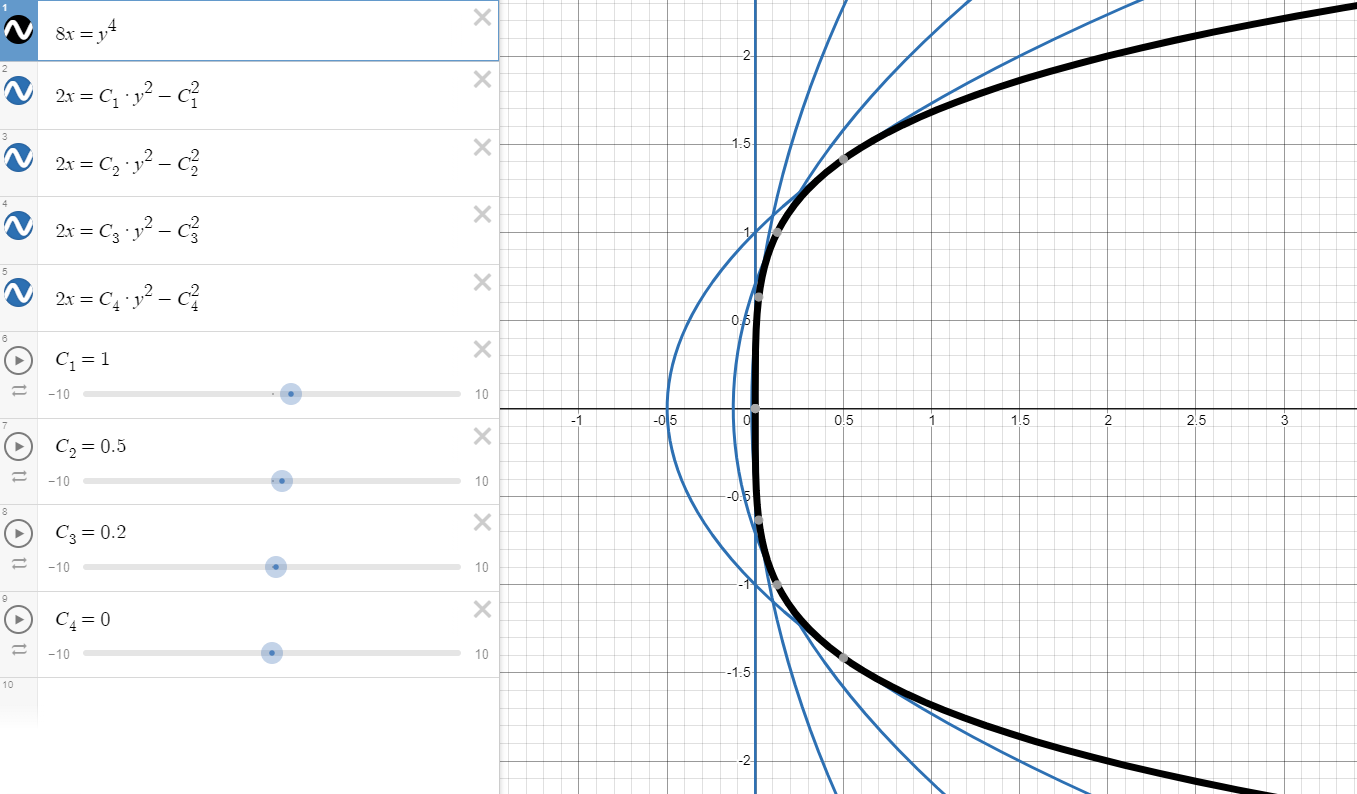
\includegraphics[width=1\linewidth]{6.36.png}}
\caption{Интегральные кривые С. \S6: 36}
\label{fig:6.36}
\end{figure}
\newline
Весьма очевидно, что особым решением, дискриминантной кривой в данном случае будет $8x=y^4$ но, к сожалению, это необходимо доказать :(
\begin{proof}
Необходимое условие дискриминантной кривой:
\begin{equation}
    \begin{cases}
    \frac{\partial}{\partial p}(2 x y^2 p^2 - y^3 p + 1) = 0\\
    2 x y^2 p^2 - y^3 p + 1 = 0\\
    \end{cases}
\end{equation}
Откуда:
\begin{equation}
    \begin{cases}
    p=\frac{y}{4 x}\\
    8x=y^4\\
    \end{cases}
\end{equation}
Как мы видим дискриминантной кривой может быть только $x=y^4/8$, но то что она таковой является надо ещё проверить:
\begin{equation}
    \begin{cases}
    \frac{d}{d y}(\frac{C y^2 - C^2}{2})=\frac{d}{d y}(y^4/8)\\
    \frac{C y^2 - C^2}{2}=y^4/8\\
    \end{cases}
\end{equation}
Что в итоге даёт:
\begin{equation}
    \begin{cases}
    C=\frac{y^2}{2}\\
    0=0
    \end{cases}
\end{equation}
Т.е. $x=y^4/8$ действительно дискриминантная кривая, касающаяся решений  вида $C y^2 - C^2$ при $C \geq 0$
\end{proof}


\subsection{С. \S6: 49 }
Решение полностю аналогично предыдущему, однако в этот раз разрешим уравнение относительно $y$ а не $x$ (это чтобы я не совсем уж весь код копипастил):
В уравнении 
\begin{equation}
    y'-\ln(y')=y-x 
\end{equation}
Сделаем замену $\frac{d y}{d x}=p$ и разрешим первое уравнение относительно $y$ 
\begin{equation}
    \begin{cases}
        y=p - \ln(p) + x\\
        \frac{d y}{d x}=p
    \end{cases}
\end{equation}
Второе уравнение системы (20) можем записать как $dy = p dx$, от первого возьмём дифференциал.
\begin{equation}
    \begin{cases}
        (p-1)(d p - p d x)=0 \\
        \frac{d y}{d x}=p
    \end{cases}
\end{equation}
Откуда:
\begin{equation}
    \begin{cases}
    \left[
    \begin{gathered}
        p=1\\
        \frac{d p}{p} = dx \\
    \end{gathered}
    \right. \\
        y=p - \ln(p) + x \\
    \end{cases}
\end{equation}
проинтегрируем второе выражение в совокупности (получим $p=e^{x+C}$) и подставим оба уравнения совокупности в уравнение на y:
\begin{equation}
\begin{cases}
\left[
\begin{gathered}
    y=1+x\\
    y=e^{x + C} -C \\
\end{gathered} \right. \\
    y=p - \ln(p) + x \\
\end{cases}
\end{equation}
Построим графики полученных кривых Рис. \ref{fig:6.49}
\begin{figure}[ht]
    \center{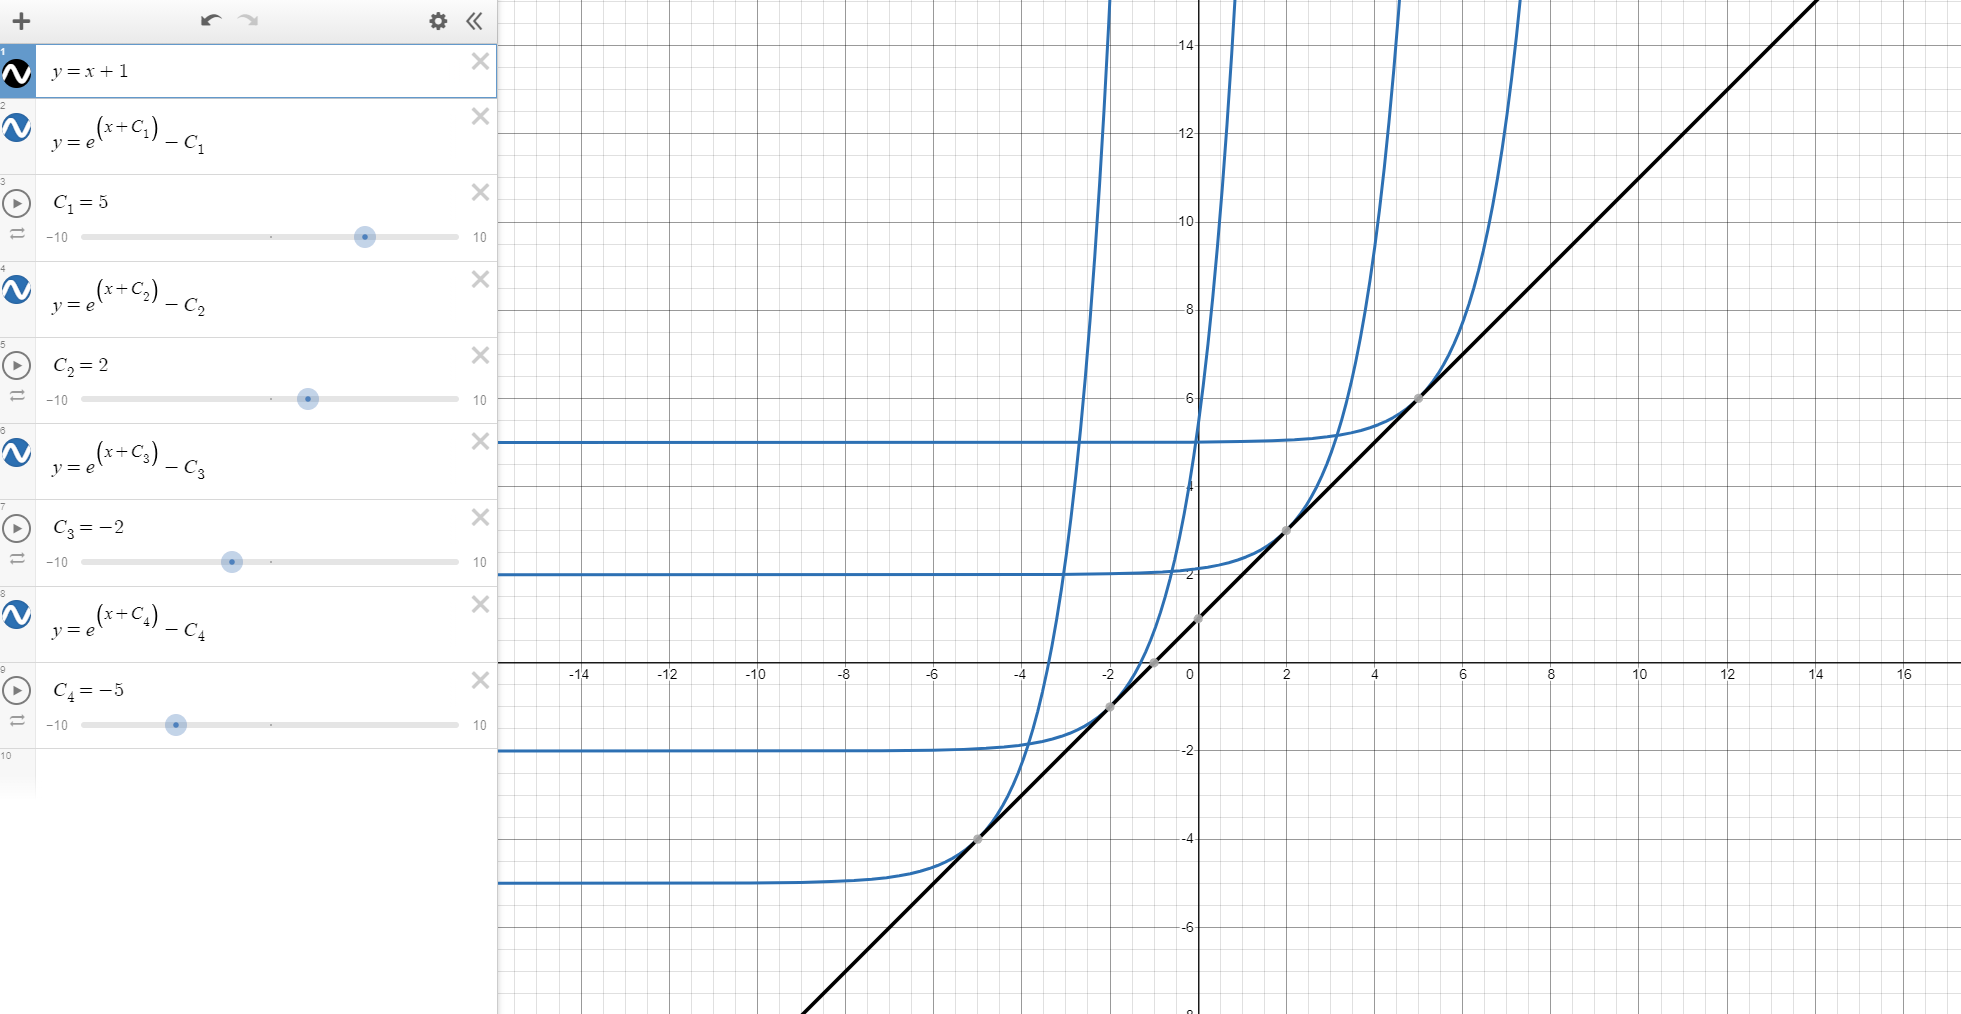
\includegraphics[width=1\linewidth]{6.49.png}}
    \caption{Интегральные кривые С. \S6: 49}
    \label{fig:6.49}
\end{figure}
\newline
Весьма очевидно, что особым решением, дискриминантной кривой в данном случае будет $y=x+1$ но, к сожалению, это необходимо доказать :(
\begin{proof}
Необходимое условие дискриминантной кривой:
\begin{equation}
    \begin{cases}
    \frac{\partial}{\partial p}(p - \ln(p) + x - y) = 0\\
    p - \ln(p) + x -y=0\\
    \end{cases}
\end{equation}
Откуда:
\begin{equation}
    \begin{cases}
    p=1\\
    y=x+1\\
    \end{cases}
\end{equation}
Как мы видим дискриминантной кривой может быть только $y=x+1$, но то что она таковой является надо ещё проверить:
\begin{equation}
    \begin{cases}
    \frac{d}{d x}(e^{x+C}-C)=\frac{d}{d x}(x+1)\\
    e^{x+C}-C=x+1\\
    \end{cases}
\end{equation}
Что в итоге даёт:
\begin{equation}
    \begin{cases}
    x+C=0\\
    0=0
    \end{cases}
\end{equation}
Т.е. $y=x+1$ действительно дискриминантная кривая, касающаяся решений  вида $e^{x+C}-C$ уже (в сравнении с предыдущей задачей) при любых $C$
\end{proof}

\subsection{Ф.: 1065}
Для решения задач 1065-1067 воспользуемся следующим фактом (Филиппов с. 109-110) :\\
Если в системе уравнений 
\begin{equation}
\label{eq2}
    \frac{d x_i}{d t} = f_i(t,x_1, ... , x_n, \mu) 
\end{equation}

с начальными условиями $x_i(0)=a_i(\mu)$ для $i=1,..,n$ \\
$\mu$ является параметром, функции $f_i$ и $a_i$ непрерывны и имеют непрерывные производные по $x_1, ... , x_n, \mu$ , то решение имеет непрерывную производную по параметру $\mu$, а производные $\frac{\partial x_i}{\partial \mu} = u_i$ удовлетворяют линейной системе уравнений \ref{eq1}:
\begin{equation}
\label{eq1}
    \frac{d u_i}{d t} = \sum_{j=1}^n \frac{\partial f_i}{\partial x_j} u_j + \frac{\partial f_i}{\partial \mu}
\end{equation}
и начальным условиям $u_i(0)=a'_i(\mu)$. Значения производных в формуле \ref{eq1} берутся при $x_i=x_i(t)$ - решения системы \ref{eq2} с заданными начальными условиями.\\

Теперь можно порешать задачи:
\begin{equation}
    y'=2x+\mu y^2
\end{equation}
с начальными условиями: $y(0)=\mu-1$. \\
Очевидно решение 
\begin{equation} \label{eq3}
    y(\mu=0)=x^2-1
\end{equation} 
Рассмотрим теперь решение в нуле уравнения \ref{eq1}. Подставим туда очевидное нам решение \ref{eq3} и получим:
\begin{equation} \label{eq4}
    \frac{d u}{d x} = x^4 - 2x^2 +1
\end{equation}
Проинтегрируем \ref{eq4} и получим:
\begin{equation}
    u(x)=x^5/5+2 x^3 /3 + x + C
\end{equation}
Поскольку $u(0)=\frac{d }{d \mu} y(0)=1$ финальным ответом будет:\\
\begin{equation}
    u=x^5/5+2 x^3 /3 + x + 1
\end{equation}
\subsection{Ф.: 1066}
\begin{equation}
    y'= y + y^2 +x y^3
\end{equation}
с начальными условиями: $y(2)=y_0$. \\
Запишем \ref{eq1} для данной задачи:
\begin{equation} \label{eq5}
    \frac{d u}{d x}=(1+2 y + 3x y^2)u
\end{equation}
Подставим в \ref{eq5} начальные условия при которых нас просят найти u: $y=y_0=0$. Проинтегрируем и получим :
\begin{equation}
    u(x)=e^{x+c}
\end{equation}
Осталось только найти константу C. Это тоже не очень трудно: $u(2)=1$ (в качестве $\mu$ мы использовали $y_0$ а значит производная, очевидно, 1). Значит $C = -2$. И конечный ответ:
\begin{equation}
u(x)=e^{x-2}
\end{equation}
\subsection{Ф.: 1067*}
Чтобы скопипастить 1065, ничего не меняя, обозначим $x$ как $y$, $t$  как $x$ 
\begin{equation}
    y'=y/x+\mu x e^{-y}
\end{equation}
с начальными условиями: $y(1)=1$. \\
Очевидно решение 
\begin{equation} \label{eq6}
    y(\mu=0)=x
\end{equation} 
Рассмотрим теперь решение в нуле уравнения \ref{eq1}. Подставим туда очевидное нам решение \ref{eq6} и $\mu=0$ получим:
\begin{equation} \label{eq7}
    \frac{d u}{d x} = u/x + x e^{-x}
\end{equation}
Решим \ref{eq7} и получим:
\begin{equation}
    u(x)= x(C - e^{-x})
\end{equation}
Поскольку $u(1)=0$ (начальные условия от мю не зависят), вернув оригинальные обозначения получим ответ:\\
\begin{equation}
    u(x)= t(e^{-1} - e^{-t})
\end{equation}
\subsection{Т1}
Ну а чего бы ему продолжаться?
\begin{proof}
рассмотрим случай $y>0$ для него решение принимает вид:
\begin{equation}\label{eq8}
    y_1=(\alpha -1)^{\frac{1}{1-\alpha}}(C_1-x)^{\frac{1}{1-\alpha}}
\end{equation}
При $y<0$ решения принимают вид:
\begin{equation}\label{eq9}
    y_1=-(\alpha -1)^{\frac{1}{1-\alpha}}(C_2-x)^{\frac{1}{1-\alpha}}
\end{equation}
 Довольно очевидно, что \ref{eq8} и \ref{eq9} не могут быть продолжены на интервал $(-\infty, + \infty)$ хотя бы из-за того что они не определены на всём интервале. Взять же объединение этих решений невозможно, потому что единственная точка, где они могли бы пересекаться: $y=0$ не достигается ни одним из решений, т.е. объединение решений никогда не будет непрерывной функцией.
\end{proof}

\subsection{T2}
Слишком много пунктов а смысла маловато $\Rightarrow$ плохая задача.\\
Решим квадратное уравнение относительно $y'$, откуда можно получить:
\begin{equation}
    \left[
\begin{gathered}
    y'=1 \\
    y'=y \\
\end{gathered}\\
\right.
\end{equation}
Тогда решениями уравнения будут кривые:
\begin{equation}\label{eq9_}
    \left[
\begin{gathered}
    y_1=x+C_1 \\
    y_2=e^{x+C_2} \\
\end{gathered}\\
\right.
\end{equation}
Покажем, что черезх каждую точку кривой $y=1$ проходит 2 кривые, имеющие общую касательную (производную). Просто приведём пример $C_1(x)$ $C_2(x)$(не следует понимать что $C_1$ и $C_2$ перестали быть константами для кривой, мы лишь смотрим какие константы соответсвуют кривым, проходящим через точку $(x,1)$. 
$e^{x+C_2}=x+C_1=1$ $\Rightarrow $
$\begin{cases} 
C_1=1-x \\ 
C_2=-x
\end{cases}, $
 тогда   $y_1'=y_2'=1$ что соответсвует наличию общей касательной.\\
Решим краевую задачу $y(0)=0, y(2)=e$. Тогда, очевидно из \ref{eq9_} $C_1=0; C_2=-1$. Построим график полученного решения \ref{fig:T2}

\begin{figure}[ht]
\center{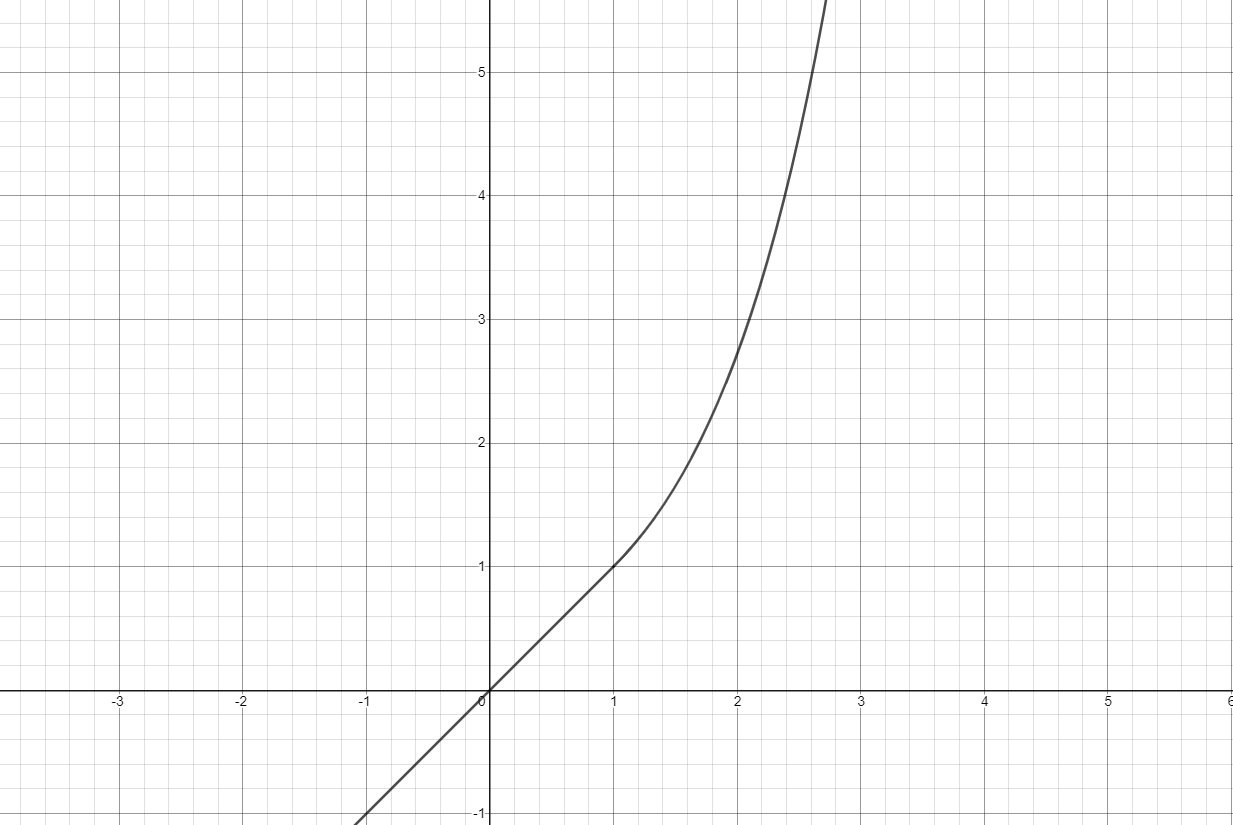
\includegraphics[width=1\linewidth]{T2.png}}
\caption{Решение краевой задачи Т2}
\label{fig:T2}
\end{figure}
\section{Линейные уравнения с переменными коэффициентами}
\subsection{Ф.: 649}
Провероить, являются ли функции $x$, $e^x$, $x e^x$ линейно независимыми на $I=(-\infty,+\infty)$.\\

Метод 1:\\ 
Воспользуемся следующим свойством определителя Вронского: Если функции $f_1(x),...,f_n(x)$ линейно зависимы на $I$, определитель Вронского $W(x)=0$ $\forall x \in I$ (обратное не обязательно верно). Откуда очевидно, что если хотя бы в 1 точке $I$ Вронскиан не 0, то функции линейно независимы (а если W(x) всюду 0, ещё нет гарантии, что функции линейно зависимы, это ещё необходимо проверить).\\
\begin{equation}\label{f649.1}
    W(x) = 
    \begin{vmatrix}
    x && e^x && e^x x \\
    1 && e^x && e^x(x+1)\\
    0 && e^x && e^x(x+2)
    \end{vmatrix}
    =x e^{2x} ((x+2)-(x+1))-1 e^{2x}((x+2)-x) = e^{2x}(x-2)
\end{equation}
Весьма очевидно, выражение \ref{f649.1} $\neq 0$ на всём промежутке $I=(-\infty,+\infty)$, а значит функции линейно независимы.\\

Метод 2: (на самом деле он не нужен для понимания материала, я вообще хз, зачем его написал, но не стирать же):\\
Предположим, фунции линейно зависимы. Тогда:
\begin{equation}\label{f649.2}
    \lambda_1 x + \lambda_2 e^x + \lambda_3 x e^x = 0 \text{ } \forall x \in I
\end{equation}
Поскольку \ref{f649.2} верно для любых $x$ подставим $x=0$,$x=1$,$x=2$, Получим систему:
\begin{equation}
    \underbrace{
    \begin{pmatrix}
    0 && 1 && 0\\
    1 && e && e\\
    2 && e^2 && 2e^2
    \end{pmatrix}}_{A}
    \begin{pmatrix}
    \lambda_1\\
    \lambda_2\\
    \lambda_3
    \end{pmatrix}
    =0
\end{equation}
 Поскольку $det(A)=2 e - 2 e^2 \neq 0$ система имеет только тривиальное решение. Противоречие. 
 \subsection{Ф.: 664}
 Еслич честно, не понимаю смысл задачи. Очевидно, функции линейно независимы, ну докажу что ли...
 \begin{proof}
Предположим функции линейно зависимы, тогда вронскиан тождественно равен нулю на всём промежутке. В то же время в точке $x_1$ $w(x) \neq 0$. Противоречие. Значит функции линейно независимы. 
 \end{proof}

\subsection{Ф.: 667}
Илья Викторович-таки попал в задачу из задания :)
Легко видеть (особенно если решать задачу сразу после семинара где она обсуждалась), что Вронскиан равен нулю. Тем не менее, это ещё не означает, что функции линейно зависимы. Покажем что это не так. Тогда воспользуемся методом 2:
Предположим, фунции линейно зависимы. Тогда:
\begin{equation}\label{f649.2_}
    \lambda_1 x + \lambda_2 x^5 + \lambda_3 |{x^5}| = 0 \text{ } \forall x \in I
\end{equation}
Поскольку \ref{f649.2_} верно для любых $x$, подставим $x=-1/2$,$x=1/4$,$x=1/2$, Получим систему:
\begin{equation}
    \underbrace{
    \begin{pmatrix}
    -1/2 && -1/32 && 1/32\\
    1/4 && 1/1024 && 1/1024\\
    1/2 && 1/32 && 1/32
    \end{pmatrix}}_{\text{ЫуЫа}}
    \begin{pmatrix}
    \lambda_1\\
    \lambda_2\\
    \lambda_3
    \end{pmatrix}
    =0
\end{equation}
 Поскольку $\det(\text{ЫуЫа})=15/32768 \neq 0$ система имеет только тривиальное решение. Противоречие. Значит функции линейно независимы.
 \subsection{Ф.: 668*}
 \begin{proof}

 В данной задаче рассматривается Вронскиан однородного дифф. уравнения 2 порядка. Это весьма важно, т.к. Определитель Вронского однородного дифференциального уравнения либо тождественно равен нулю, и это означает, что $f_{1}(x),\ldots ,f_{n}(x)$ линейно зависимы, либо не обращается в нуль ни в одной точке $I$, что означает линейную независимость функций $ f_{1}(x),\ldots ,f_{n}(x)$. Пусть $g(x)$, $h(x)$ - те самые 2 решения из условия. Тогда:
 \begin{equation}
     W(x)=
     \begin{vmatrix}
      g(x) && p(x) \\
      g'(x) && p'(x)
     \end{vmatrix}
 \end{equation}
Кроме того мы знаем, что в некоторой точке эти функции имеют максимум, т.е. $\exists x_0:$ $g'(x) = p'(x) = 0$ Тогда Вронскиан в $x_0$:
 \begin{equation}
     W(x)=
     \begin{vmatrix}
      g(x_0) && p(x_0) \\
      0 && 0
     \end{vmatrix}
     =0
 \end{equation}
 Что означает линейную зависимость $g(x)$ и $h(x)$.
\end{proof}
Стоит отметить, что если бы функции $g(x)$ и $h(x)$ были не решениями однородного дифф. уравнения 2 порядка, а просто какими-то функциями, то такое доказательство не было бы верно, например: $g(x)=\cos(x)$ $h(x)=-x^2+\pi$ имеют максимум в $(0,0)$, но очевидно линейно независимы.
\subsection{Ф.: 673}
Пристально посмотрим на решения $y_1=x^2-2x+2$, $y_2=x^2-4x+4$, $y_3=x^2+x-1$, $y_4=-x-1$. Можно заметить, что: $y_3+3 y_4=y_1$, $y_3+5 y_4=y_2$. Решения $y_3, y_4$ очевидно линейно независимы. Знгачит есть только 2 линейно независимых решения. Пусть $y(x)$ - общее решение диф уравнения. Оно всегда будет линейно зависимо с частными. Тогда:
\begin{equation}\label{f673.1}
    W(x)=
    \begin{vmatrix}
     y(x)&& y_3 && y_4\\
     y'(x)&& y_3' && y_4'\\
     y''(x)&& y_3'' && y_4''
    \end{vmatrix}
    =0
\end{equation}
Равенство \ref{f673.1} это уже пример д.у. второго порядка. Т.е. $N_{min} \leq 2$. Очевидно, $N_{min} \neq 1$ Потому что у д.у. первого порядка не может быть 2 линейно независимых решений. Откуда получаем ответ: $N\geq 2$
\subsection{Ф.: 678}
Воспользуемся методом из предыдущей задачи: скажем что общее решение д.у. всегда линейно зависимо с наибольшей по включению линейно независимой системой частных решений этого д.у., а значит Вронскиан $W(y(x),f_1,\ldots, f_n)=0$\\
$y_1(x)=sh(x)$ $y_1'(x)=ch(x)$ $y_1(x)''=sh(x)$ \\
$y_2(x)=ch(x)$ $y_2'(x)=sh(x)$ $y_2(x)''=sh(x)$ \\
$y_3(x)=e^x=y_1(x)+y_2(x)$ это решение не надо писать во Вронскиане, поскольку оно уже линейно зависимо с другими 2\\
Тогда построим д.у.:
\begin{equation}
    W(x)
    =
    \begin{vmatrix}
     y(x) && sh(x) && ch(x)\\
     y'(x) && ch(x) && sh(x)\\
     y''(x) && sh(x) && ch(x)\\
    \end{vmatrix}
    =y''(x) (sh^2(x)-ch^2(x)) - y'(x) (sh(x)ch(x)-sh(x)ch(x)) + y(x) (ch^2(x)-sh^2(x))
    =0
\end{equation}
И итоговое д.у. получается весьма красивым: $y''(x)-y(x)=0$
\subsection{Ф. \S22:47*}
Рассмотрим уравнение 
\begin{equation} \label{22:47.1}
(x+2)y''-3y'+y \sqrt{1-x}=0    
\end{equation}
Выражение \ref{22:47.1} запишем в приведённом виде.
\begin{equation}
    y''- \frac{3y'}{(x+2)} + \frac{y \sqrt{1-x}}{x+2}=0 
\end{equation}
а)Т.к. коэффициенты непрерывны только на промежутке $(-2,1]$ то решения можно продолжить не более чем на этот промеждуток. Это оценка сверху. Теперь осталось доказать что решения действительно можно продолжить...
б) в точке 0 детерминант Вронского
\begin{equation*}
W(x=0)=
\begin{vmatrix}
y_1(0) && y_2(0)\\
y_1'(0) && y_2'(0)\\
\end{vmatrix}
=
\begin{vmatrix}
1 && 3\\
0 && 2\\
\end{vmatrix}
= 2 \neq 0
\end{equation*}
Не равен нулю, а значит решения $y_1(x)$ и $y_2(x)$ линейно независимы и составляют фундаментальную систему.
в) Для нахождения $W(x=-1)$ воспользуемся формулой Лиувилля — Остроградского: \\
Пусть есть уравнение вида:
\begin{equation}
    y^{(n)}+P_{1}(x)y^{(n-1)}+P_{2}(x)y^{(n-2)}+...+P_{n}(x)y=0,
\end{equation}
тогда:
\begin{equation}
    W(x)=W(x_0) e^{-\int_{x_0}^x P_1(t)dt}
\end{equation}
Тогда для нашей задачи:
\begin{equation}
    W(x=-1)=W(x_0) e^{-\int_{x_0}^{-1} P_1(t)dt}=2 e^{-\int_{0}^{-1} \frac{-3}{t+2}dt}=2 e^{-\ln(8)}=1/4
\end{equation}
\subsection{Ф. \S22:59}
Обозначим искомое решение как $y_{\text{ЫуЫа}}$
Т.к. известны три частных, можем найти базисные решения, как разность частных:\\
$\varphi_1=y_1-y_2 = x^2+x-1$\\
$\varphi_2=y_2-y_3 = 2x$\\
Таким образом общее решение Д.У. будет иметь вид:
\begin{equation}
    y(x)=C_1\varphi_1+C_2\varphi_2+y_1=C_1(x^2+x-1)+C_2x+x^2
\end{equation}
и, очевидно:
\begin{equation}
    y'(x)=C_1(2x+1)+C_2+2x
\end{equation}
Здесь двойку из решения $\varphi_2$ я внёс под константу, ну потому что лень с ней работать.\\
Подберём теперь константы $C_1$ и $C_2$ для наших начальных условий.
\begin{equation}
    y(0)=2=C_1(0^2+0-1)+0 C_2+0^2=-C_1
\end{equation}
\begin{equation}
    y'(0)=0=C_1(2\cdot 0+1)+C_2+2 \cdot 0=C_1+C_2
\end{equation}
Таким образом: $C_1=-2$ и $C_2=2$, откуда: $y_{\text{ЫуЫа}}=-x^2+2$
\subsection{С. \S9: 10 }
Решить уравнение 
\begin{equation}
    2 x y'' + (4x+1)y' + (2x+1)y=e^{-x}, x>0
\end{equation}
1) угадаем первое решение О.Д.У в виде $\varphi_1(x)=e^{\alpha x}$.
\begin{equation}
    2x e^{\alpha x} \alpha^2 + (4x+1)e^{\alpha x}\alpha + (2x+1) e^{\alpha x}=0
\end{equation}
Приводя подобные слагаемые получим:
\begin{equation}
    \begin{cases}
    x(\alpha^2+2 \alpha +1)=0   \\
        \alpha +1 =0
    \end{cases}
\end{equation}
Откуда, очевидно следует что 1) мы угадали одно решение 2) $\alpha =-1$ $\Rightarrow$ $\varphi_1=e^{-x}$
Теперь надо найти второе решение однородного. Запишем формулу Остроградского - Лиувилля в удобном нам виде:
\begin{equation}
    \frac{d}{dx} \left( \frac{y_o}{\varphi_1} \right)= \frac{C}{\varphi_1^2} \exp \left( - \int \frac{4x+1} {2x}dx  \right) 
\end{equation}
\textcolor[rgb]{1,1,1}{Где-то здесь я понял, что нумеровать абсолютно все (ну или почти все) формулы эстетически не очень красиво, поскольку как-то их многовато, а я на них не особо-то сылаюсь, но дороги назад уже не было. }
\begin{equation}
    \frac{d}{dx} \left( \frac{y_o}{e^{-x}} \right)= \frac{C}{e^{-2x}} \exp \left(-2x - \frac{\ln(x)}{2}  \right) = C x^{-1/2}
\end{equation}
Проинтегрировав получим $y_o=C_1 \underbrace{e^{-x}}_{\varphi_1}+ C_2 \underbrace{e^{-x} \sqrt x}_{\varphi_2}$. 
Для нахождения решение неоднородного Д.У. воспользуемся методом вариации постоянной. 
Ищем решение в виде:$y(x)=C_1(x)\varphi_1 + C_2(x) \varphi_2$. $C_1(x)$ и $C_2(x)$ найдём из системы
\begin{equation}
    \begin{cases}
        C_1' \varphi_1+C_2'\varphi_2=0\\
        C_1' \varphi_1'+C_2'\varphi_2'=\frac{e^{-x}}{2x}
    \end{cases}
\end{equation}
Подставим всё, чутка упростим и получим:
\begin{equation}
    \begin{cases}
        C_1'+C_2' \sqrt x = 0\\
        -C_1'+C_2' \sqrt x (\frac{1}{2x}-1)=C_2 \frac{\sqrt x }{2x}=1/2x
    \end{cases}
\end{equation}
Решая систему получим: $C_1(x)= -x + C_1$ $C_2(x)=2 \sqrt x + C_2$. Осталось только подставить всё в исходное уравнение и получить: $y_o=C_1 e^{-x}+C_2\sqrt x e^{-x} + x e^{-x}$ 

\subsection{С. \S9: 31 }
ну тут алгоритм +- понятен я попозже сделаю...
\subsection{С. \S9: 53 }
ну тут алгоритм +- понятен я попозже сделаю...
\subsection{С. \S9: 64 }
ну тут алгоритм +- понятен я попозже сделаю...
\subsection{С. \S9: 68(а)}
попооозже
\subsection{Т3} 
\begin{proof}
Предположим, существуют линейно независимые $y_1$ , $y_2$ ограниченные вместе со своими производными. Тогда, в любой положительной окрестности 0, Вронскеан этих функций не 0, кроме того он обязан быть ограничен, поскольку ограничены сами функции и их первые производные. Для любой положительной $\varepsilon$-окрестности точки 0 внутри неё возьмём некоторую точку $\delta$. Т.к. Вронскеан не ноль, положим $W(\varepsilon)=W_0$ Запишем формулу Лиувилля - Остроградского:
\begin{equation}
    W(\delta)=W_0 \exp \left(- \int^{\delta}_{\varepsilon} \frac{x}{x^2} \, dx  \right) = W_0 \frac{\varepsilon}{\delta}
\end{equation}
Ну тут уже становится очевидно, что если в любой окрестности нуля вронскеан не 0 хотя бы в одной точке, он начинает неограниченно возрастать при стремлении к 0:\\
$\forall  \varepsilon > 0 \forall M \exists \delta =  \frac{\varepsilon}{2|M|}: W(\delta)>|M|$
А раз Вронскеан не ограничен, чего бы производным и функциям оказаться ограниченными?
\end{proof}



\end{document}
